\documentclass[12pt]{article}

\usepackage{report-template}

% Disable indentation on new paragraphs
\setlength{\parindent}{2em}

% Line spacing 1.5
\renewcommand{\baselinestretch}{1.5}

% Optional: graphic path
% \graphicspath{PATH_TO_GRAPHIC_FOLDER}

% To use Times font family, uncomment this row
% \usepackage{mathptmx}

% To use roman section / subsection, uncomment these rows
% \renewcommand{\thesection}{\Roman{section}}
% \renewcommand{\thesubsection}{\thesection.\Roman{subsection}}

% Define course name, report name and report title.
\newcommand{\coursename}{Khai phá Dữ liệu}
\newcommand{\reportname}{XÂY DỰNG HỆ THỐNG KHO DỮ LIỆU VÀ KHAI PHÁ DỮ LIỆU CHO LĨNH VỰC HÀNG KHÔNG}
\newcommand{\reporttitle}{BÁO CÁO BÀI TẬP LỚN}

\newcommand{\studentname}{Đoàn Trí Hùng (2211322)\\Nguyễn Mạnh Hùng (2211337)\\Nguyễn Cao Cường (2210429)}
\newcommand{\teachername}{Thầy Đỗ Thanh Thái}

% Header
\lhead{\reporttitle}
\rhead{
Trường Đại học Bách Khoa Hồ Chí Minh - ĐHQG HCM\\
\coursename
}

% Footer
% \newcommand{\leftfooter}{\LaTeX\ by \href{https://github.com/trhgquan}{Quan, Tran Hoang}}
% \lfoot{\leftfooter}

% ============ DOCUMENT ============
\begin{document}

\pagenumbering{roman}
\begin{titlepage}
\newcommand{\HRule}{\rule{\linewidth}{0.5mm}}
\centering

\textsc{\LARGE đại học quốc gia tphcm}\\[0.5cm]
\textsc{\Large trường đại học bách khoa hồ chí minh}\\[0.5cm]
\textsc{\large khoa khoa học và kỹ thuật máy tính}\\[0.5cm]


\includegraphics[scale=0.5]{img/hcmut-logo.png}\\[0.5cm] 

\HRule \\[0.4cm]
{ 
\huge{\bfseries{\reporttitle}}\\[0.5cm]
\large{\bfseries{ĐỀ TÀI: \reportname}}
}\\[0.4cm]
\HRule \\[0.5cm]

\textbf{\large Môn học: \coursename}\\[0.5cm]

\begin{minipage}[t]{0.4\textwidth}
\begin{flushleft} \large
\emph{Sinh viên thực hiện:} \\
\studentname
\end{flushleft}
\end{minipage}
~
\begin{minipage}[t]{0.4\textwidth}
\begin{flushright} \large
\emph{Giáo viên hướng dẫn:} \\
\teachername
\end{flushright}
\end{minipage}\\[1cm]

Link source code: \href{https://github.com/hungdt31/airline-dw-system}{https://github.com/hungdt31/airline-dw-system} \\
{\large \today}

\vfill
\end{titlepage}
	

% ============================================================
% BẢNG PHÂN CHIA CÔNG VIỆC
% ============================================================
\thispagestyle{plain}
\begin{center}
  {\large\bfseries BẢNG PHÂN CHIA CÔNG VIỆC}
\end{center}

\begin{tabular}{|c|l|c|p{5.5cm}|p{2.5cm}|}
\hline
\textbf{STT} & \textbf{Họ và Tên} & \textbf{MSSV} & \textbf{Nhiệm vụ} & \textbf{Phần trăm hoàn thành} \\
\hline
1 & Đoàn Trí Hùng  & 2211322 &
  Xây dựng pipeline ETL, thiết kế Star Schema (SQLite),
  phát triển Dashboard Streamlit 6 trang,
  viết báo cáo.
  & 100\% \\
\hline
2 & Nguyễn Mạnh Hùng & 2211337 &
  Huấn luyện và so sánh 5 mô hình ML
  (Logistic Regression, Random Forest, Neural Network,
  XGBoost, LightGBM),
  phân tích kết quả, Feature Importance.
  & 100\% \\
\hline
3 & Nguyễn Cao Cường & 2210429 &
  Khảo sát dữ liệu nguồn,
  xây dựng bộ truy vấn OLAP,
  tổng hợp tài liệu tham khảo, làm slide thuyết trình.
  & 100\% \\
\hline
\end{tabular}

\pagebreak

\tableofcontents
\pagebreak
\listoftables
\pagebreak
\listoffigures
\pagebreak

\pagenumbering{arabic}
\setcounter{page}{1}

% ============================================================
% CHƯƠNG 1: TỔNG QUAN ĐỀ TÀI
% ============================================================
\section{Tổng quan đề tài}

\subsection{Vấn đề đặt ra}

\subsubsection{Thực trạng trì hoãn chuyến bay tại Mỹ năm 2015}

Theo dữ liệu của Cục Hàng không Liên bang Mỹ (FAA), năm 2015 ghi nhận hơn 5,8 triệu chuyến bay nội địa,
trong đó xấp xỉ 21\% bị trì hoãn (delay) với thời gian trễ trên 15 phút.
Tình trạng này gây thiệt hại kinh tế ước tính hàng tỷ đô la mỗi năm, bao gồm chi phí nhiên liệu tăng thêm,
bồi thường hành khách, và ảnh hưởng đến lịch trình của toàn bộ hệ thống hàng không.

Các nguyên nhân chính gây delay được ghi nhận bao gồm:
\begin{itemize}
    \item \textbf{Thời tiết} (Weather Delay): Bão, sương mù, tuyết rơi ảnh hưởng đến tầm nhìn và khả năng cất hạ cánh.
    \item \textbf{Hệ thống quản lý không lưu} (NAS Delay): Tắc nghẽn không phận, hạn chế đường bay.
    \item \textbf{Vận hành của hãng hàng không} (Carrier Delay): Sự cố kỹ thuật, thiếu phi hành đoàn.
    \item \textbf{Tàu bay đến muộn} (Late Aircraft Delay): Hệ quả dây chuyền từ chuyến bay trước bị delay.
    \item \textbf{An ninh} (Security Delay): Kiểm tra an ninh kéo dài.
\end{itemize}

\subsubsection{Hạn chế của các phân tích thủ công truyền thống}

Các phương pháp phân tích truyền thống dựa trên báo cáo tĩnh, bảng tính Excel hoặc truy vấn SQL đơn giản
gặp phải nhiều hạn chế khi xử lý tập dữ liệu ở quy mô hàng triệu bản ghi:
\begin{itemize}
    \item Không thể phân tích đa chiều (theo hãng, sân bay, tháng, ngày trong tuần) một cách linh hoạt.
    \item Thiếu khả năng phát hiện mẫu ẩn (hidden patterns) trong dữ liệu lớn.
    \item Không dự báo được xác suất delay cho chuyến bay mới trước khi xảy ra.
    \item Chi phí xử lý cao và thời gian phân tích kéo dài khi dữ liệu tăng lên.
\end{itemize}

\subsubsection{Nhu cầu có hệ thống phân tích tự động và dự báo}

Để giải quyết bài toán trên, cần một hệ thống tích hợp có khả năng:
\begin{enumerate}
    \item Tự động thu thập, làm sạch và lưu trữ dữ liệu hàng không theo chuẩn Data Warehouse.
    \item Cung cấp giao diện phân tích OLAP đa chiều, cho phép drill-down/roll-up theo nhiều chiều dữ liệu.
    \item Áp dụng các thuật toán Machine Learning để dự báo khả năng delay của chuyến bay mới.
\end{enumerate}

% ------------------------------------------------------------
\subsection{Mục tiêu}

Đề tài hướng đến ba mục tiêu chính:

\begin{enumerate}
    \item \textbf{Xây dựng Data Warehouse chuẩn hóa dữ liệu hàng không:}
    Thiết kế và triển khai kho dữ liệu theo mô hình Star Schema với bảng sự kiện \texttt{fact\_flights}
    và các bảng chiều \texttt{dim\_airline}, \texttt{dim\_airport}, \texttt{dim\_date}, \texttt{dim\_time},
    đảm bảo tính nhất quán và khả năng truy vấn hiệu quả.

    \item \textbf{Cung cấp dashboard phân tích OLAP đa chiều:}
    Xây dựng dashboard tương tác 2 cấp phân tích --- cấp tổng quan (tỷ lệ delay theo hãng, sân bay, tháng)
    và cấp nguyên nhân (phân tích chi tiết từng loại delay) --- cho phép người dùng lọc động theo nhiều tiêu chí.

    \item \textbf{Dự báo khả năng delay chuyến bay mới:}
    So sánh và đánh giá 5 thuật toán phân loại (Logistic Regression, Random Forest, Neural Network,
    XGBoost, LightGBM) trên cùng tập dữ liệu, chọn ra mô hình tốt nhất để dự báo delay.
\end{enumerate}

% ------------------------------------------------------------
\subsection{Phạm vi}

\paragraph{Dữ liệu:}
Đề tài sử dụng bộ dữ liệu \textit{US Flight Delays 2015} công khai trên Kaggle \cite{kaggle2015},
bao gồm ba file CSV:
\begin{itemize}
    \item \texttt{flights.csv}: 5.819.079 chuyến bay, 31 thuộc tính (thời gian, hãng bay, sân bay, các loại delay).
    \item \texttt{airlines.csv}: Thông tin 14 hãng hàng không nội địa Hoa Kỳ.
    \item \texttt{airports.csv}: Thông tin 322 sân bay (tên, thành phố, tiểu bang, tọa độ địa lý).
\end{itemize}

\paragraph{Thời gian và không gian:}
Dữ liệu bao phủ toàn bộ năm 2015 (1/1/2015 -- 31/12/2015), chỉ bao gồm các chuyến bay nội địa Hoa Kỳ.
Dữ liệu quốc tế và các năm khác nằm ngoài phạm vi của đề tài.

% ------------------------------------------------------------
\subsection{Đóng góp}

Đề tài đạt được ba đóng góp kỹ thuật chính:

\begin{enumerate}
    \item \textbf{ETL pipeline tối ưu bộ nhớ:}
    Pipeline xử lý dữ liệu theo kiểu streaming (chunk 100.000 dòng/lần) kết hợp tối ưu dtype
    (float32/int8/int16 thay cho float64/int64) và vectorized transform với \texttt{numpy.select()},
    cho phép nạp toàn bộ 5,8 triệu dòng vào SQLite với mức tiêu thụ RAM chỉ \textasciitilde{}120 MB/chunk,
    thời gian ước tính 3--8 phút tùy tốc độ ổ đĩa.

    \item \textbf{So sánh hệ thống 5 thuật toán Machine Learning:}
    Xây dựng framework đánh giá thống nhất cho 5 thuật toán (Logistic Regression, Random Forest,
    Neural Network, XGBoost, LightGBM) trên cùng tập train/test với các chỉ số AUC-ROC, F1,
    Precision, Recall và thời gian huấn luyện, cho phép so sánh khách quan và toàn diện.

    \item \textbf{Dashboard tương tác 2 cấp phân tích:}
    Giao diện Streamlit 2 tab: (1) tổng quan với 4 KPI cards và biểu đồ theo hãng/sân bay/tháng/quý,
    (2) phân tích nguyên nhân delay với pie chart, delay theo mùa và theo khung giờ bay.
    Bộ lọc động 4 chiều: thời gian, hãng bay, sân bay đi (lọc theo bang), sân bay đến (lọc theo bang).
\end{enumerate}

% ============================================================
% CHƯƠNG 2: CƠ SỞ LÝ THUYẾT
% ============================================================
\clearpage
\section{Cơ sở lý thuyết}

\subsection{Data Warehouse và OLAP}

\subsubsection{Khái niệm Data Warehouse và Star Schema}

\textbf{Data Warehouse (Kho dữ liệu)} là hệ thống lưu trữ dữ liệu tích hợp, hướng chủ đề (subject-oriented),
không biến động (non-volatile) và biến thiên theo thời gian (time-variant), được thiết kế phục vụ cho mục đích
phân tích và hỗ trợ ra quyết định \cite{inmon2005building}.
Khác với cơ sở dữ liệu tác nghiệp (OLTP) tối ưu cho giao dịch nhanh,
Data Warehouse được tối ưu cho các truy vấn phân tích phức tạp trên khối lượng dữ liệu lớn.

\textbf{Star Schema} là mô hình tổ chức dữ liệu phổ biến nhất trong Data Warehouse,
được đề xuất bởi Ralph Kimball \cite{kimball2013datawarehouse}.
Cấu trúc bao gồm:
\begin{itemize}
    \item \textbf{Fact Table (Bảng sự kiện):} Lưu trữ các chỉ số đo lường định lượng (measures)
          của sự kiện kinh doanh, ví dụ: thời gian delay, khoảng cách bay, số lượng chuyến bay.
          Fact table chứa các khóa ngoại (foreign key) trỏ đến các bảng chiều.
    \item \textbf{Dimension Tables (Bảng chiều):} Mô tả các thuộc tính ngữ cảnh của sự kiện
          (hãng bay, sân bay, thời gian, địa lý). Mỗi bảng chiều liên kết trực tiếp với fact table,
          tạo hình dạng ngôi sao đặc trưng.
\end{itemize}

So với \textbf{Snowflake Schema} --- biến thể chuẩn hóa của Star Schema trong đó các bảng chiều
được phân rã thêm --- Star Schema có ưu điểm truy vấn đơn giản hơn (ít JOIN hơn),
hiệu suất cao hơn cho các OLAP query, và dễ hiểu hơn với người dùng cuối,
với đánh đổi là dư thừa dữ liệu (data redundancy) ở mức chấp nhận được.

\subsubsection{OLAP và các phép phân tích đa chiều}

\textbf{OLAP (Online Analytical Processing)} là công nghệ cho phép phân tích dữ liệu đa chiều
một cách linh hoạt và tương tác \cite{codd1993olap}.
Dữ liệu được tổ chức thành \textit{Data Cube} --- cấu trúc đa chiều cho phép xem xét dữ liệu
từ nhiều góc độ khác nhau đồng thời.

Các phép phân tích OLAP cơ bản bao gồm:
\begin{itemize}
    \item \textbf{Roll-up:} Tổng hợp dữ liệu lên mức cao hơn trong hệ thứ bậc,
          ví dụ từ tháng $\rightarrow$ quý $\rightarrow$ năm.
    \item \textbf{Drill-down:} Phân rã dữ liệu xuống mức chi tiết hơn,
          ví dụ từ hãng bay $\rightarrow$ từng chuyến bay cụ thể.
    \item \textbf{Slice:} Cắt lát Data Cube theo một giá trị cố định của một chiều,
          ví dụ chỉ xem dữ liệu tháng 12.
    \item \textbf{Dice:} Lọc Data Cube theo nhiều điều kiện đồng thời trên nhiều chiều.
    \item \textbf{Pivot (Rotate):} Xoay trục nhìn của Data Cube để quan sát từ góc độ khác.
\end{itemize}

% ------------------------------------------------------------
\subsection{Tiền xử lý dữ liệu}

Tiền xử lý dữ liệu là bước quan trọng nhằm đảm bảo chất lượng dữ liệu đầu vào cho cả phân tích
OLAP lẫn huấn luyện mô hình khai phá. Quy trình bao gồm bốn giai đoạn chính \cite{han2011datamining}:

\subsubsection{Data Cleaning (Làm sạch dữ liệu)}

Làm sạch dữ liệu xử lý ba vấn đề chính:
\begin{itemize}
    \item \textbf{Missing values (Giá trị thiếu):} Dữ liệu hàng không có thể thiếu thông tin
          về thời gian delay khi chuyến bay bị hủy (CANCELLED = 1) hoặc chuyển hướng (DIVERTED = 1).
          Chiến lược xử lý: điền giá trị 0 cho các cột delay khi chuyến bay bị hủy
          (không có delay thực tế), loại bỏ bản ghi không xác định được nguyên nhân.
    \item \textbf{Outliers (Giá trị ngoại lệ):} Các bản ghi có thời gian delay âm
          (tàu bay đến sớm hơn dự kiến) hoặc cực lớn (>1000 phút) cần được kiểm tra và xử lý phù hợp.
          Giá trị delay âm được giữ lại (tàu đến sớm) nhưng được clip ở ngưỡng hợp lý khi feature engineering.
    \item \textbf{Inconsistency (Mâu thuẫn):} Kiểm tra tính nhất quán giữa các cột,
          ví dụ tổng thời gian delay các thành phần phải xấp xỉ tổng delay thực tế (\texttt{ARRIVAL\_DELAY}).
\end{itemize}

\subsubsection{Data Integration (Tích hợp dữ liệu)}

Tích hợp dữ liệu từ 3 nguồn CSV độc lập:
\begin{itemize}
    \item \texttt{flights.csv} $\leftarrow$ nguồn chính chứa sự kiện chuyến bay.
    \item \texttt{airlines.csv} $\leftarrow$ tra cứu tên đầy đủ hãng bay từ mã IATA.
    \item \texttt{airports.csv} $\leftarrow$ tra cứu thông tin sân bay (tên, thành phố, tiểu bang, tọa độ).
\end{itemize}
Quá trình tích hợp sử dụng lookup join trong quá trình ETL để điền thông tin
vào các bảng chiều tương ứng, tránh lưu trùng lặp trong fact table.

\subsubsection{Data Transformation (Biến đổi dữ liệu)}

\begin{itemize}
    \item \textbf{Normalization (Chuẩn hóa):} Các cột số học như \texttt{DEPARTURE\_DELAY},
          \texttt{DISTANCE}, \texttt{SCHEDULED\_DEPARTURE} được chuẩn hóa về khoảng [0, 1]
          hoặc chuẩn hóa z-score trước khi đưa vào mô hình học máy.
    \item \textbf{Feature construction (Xây dựng đặc trưng mới):}
          Tạo các đặc trưng dẫn xuất như: giờ khởi hành (0--23), tháng trong năm, ngày trong tuần,
          nhãn phân loại \texttt{is\_delayed} (1 nếu \texttt{ARRIVAL\_DELAY} $\geq$ 15 phút, 0 nếu ngược lại).
    \item \textbf{Encoding:} Các biến phân loại (mã hãng bay, mã sân bay) được mã hóa
          bằng Label Encoding hoặc Target Encoding để phù hợp với đầu vào của các thuật toán.
\end{itemize}

\subsubsection{Data Reduction (Giảm chiều dữ liệu)}

\begin{itemize}
    \item \textbf{Attribute selection (Chọn lọc thuộc tính):} Từ 31 cột trong \texttt{flights.csv},
          chọn ra 10 đặc trưng có thể biết \textit{trước khi} chuyến bay khởi hành để đảm bảo
          mô hình có thể được sử dụng thực tế (không dùng thông tin rò rỉ tương lai).
    \item \textbf{Sampling (Lấy mẫu):} Do mất cân bằng lớp (79\% không delay, 21\% delay),
          áp dụng chiến lược class\_weight để cân bằng ảnh hưởng trong quá trình huấn luyện,
          thay vì oversampling/undersampling vật lý để tránh tăng thời gian huấn luyện.
\end{itemize}

% ------------------------------------------------------------
\subsection{Các thuật toán khai phá dữ liệu}

\subsubsection{Logistic Regression}

Logistic Regression là thuật toán phân loại tuyến tính cơ bản,
mô hình hóa xác suất thuộc lớp dương theo hàm sigmoid:
\[
P(y=1 \mid \mathbf{x}) = \frac{1}{1 + e^{-(\mathbf{w}^T\mathbf{x} + b)}}
\]
Tham số $\mathbf{w}$ được tối ưu bằng Maximum Likelihood Estimation (MLE) với regularization L1/L2.
Ưu điểm: nhanh, giải thích được qua hệ số $\mathbf{w}$, xác suất đầu ra calibrate tốt.
Hạn chế: chỉ mô hình hóa được quan hệ tuyến tính.

\subsubsection{Random Forest}

Random Forest là phương pháp ensemble kết hợp nhiều Decision Tree \cite{breiman2001random}.
Mỗi cây được huấn luyện trên bootstrap sample và chỉ xét ngẫu nhiên $\sqrt{d}$ đặc trưng tại mỗi node,
làm giảm tương quan giữa các cây. Kết quả phân loại là majority vote của tất cả cây.
Random Forest có khả năng bắt được quan hệ phi tuyến và cung cấp Feature Importance tự nhiên.

\subsubsection{Neural Network (Mạng nơ-ron nhân tạo)}

Mô hình Multilayer Perceptron (MLP) với các lớp fully-connected, hàm kích hoạt ReLU ở các lớp ẩn
và sigmoid ở lớp đầu ra cho bài toán phân loại nhị phân.
Mô hình được tối ưu bằng Adam optimizer với binary cross-entropy loss.
Neural Network có khả năng học các biểu diễn đặc trưng phức tạp nhưng đòi hỏi nhiều dữ liệu
và thời gian huấn luyện hơn.

\subsubsection{Gradient Boosting: XGBoost và LightGBM}

\textbf{XGBoost} \cite{chen2016xgboost} và \textbf{LightGBM} \cite{ke2017lightgbm} là hai triển khai
hiệu quả của thuật toán Gradient Boosting Decision Trees (GBDT).
Thuật toán xây dựng cây quyết định tuần tự, mỗi cây mới học để sửa lỗi của các cây trước:
\[
F_m(\mathbf{x}) = F_{m-1}(\mathbf{x}) + \eta \cdot h_m(\mathbf{x})
\]
trong đó $h_m$ là cây mới được tối ưu để giảm residual, $\eta$ là learning rate.
LightGBM sử dụng Leaf-wise tree growth và Gradient-based One-Side Sampling (GOSS)
giúp huấn luyện nhanh hơn XGBoost trên dữ liệu lớn.

\subsubsection{Các chỉ số đánh giá}

Với bài toán phân loại nhị phân có mất cân bằng lớp, các chỉ số đánh giá bao gồm:

\begin{itemize}
    \item \textbf{AUC-ROC:} Diện tích dưới đường ROC (Receiver Operating Characteristic),
          đo khả năng phân biệt hai lớp bất kể ngưỡng quyết định. Giá trị từ 0,5 (ngẫu nhiên) đến 1 (hoàn hảo).
    \item \textbf{F1-score:} Trung bình điều hòa của Precision và Recall:
          $F_1 = 2 \cdot \frac{\text{Precision} \times \text{Recall}}{\text{Precision} + \text{Recall}}$
    \item \textbf{Precision:} Tỷ lệ dự đoán delay đúng trong tổng số dự đoán delay.
          $\text{Precision} = \frac{TP}{TP + FP}$
    \item \textbf{Recall:} Tỷ lệ chuyến bay delay thực sự được phát hiện.
          $\text{Recall} = \frac{TP}{TP + FN}$
\end{itemize}

Trong ngữ cảnh này, Recall quan trọng hơn Precision vì bỏ sót chuyến bay delay thực sự
(False Negative) gây hại lớn hơn cảnh báo nhầm (False Positive).

% ============================================================
% CHƯƠNG 3: THIẾT KẾ HỆ THỐNG  (kiến trúc logic — không đi sâu hiện thực mã)
% ============================================================
\clearpage
\section{Thiết kế hệ thống}
\label{sec:system_design}

Chương này mô tả \textbf{kiến trúc logic}: hệ thống gồm những \textbf{thành phần} nào,
mỗi thành phần \textbf{đảm nhiệm} gì và \textbf{tương tác} với nhau ra sao.
Hình~\ref{fig:system_overview} là sơ đồ trung tâm.
Việc lựa chọn công nghệ, cấu trúc thư mục mã nguồn, tham số thuật toán và đoạn lệnh cụ thể
được tập trung ở Chương~\ref{sec:implementation_experiment} (Hiện thực và thực nghiệm).

% ------------------------------------------------------------
\subsection{Kiến trúc tổng quan}

Hệ thống tổ chức theo mô hình \textbf{phân tầng}: dữ liệu thô được đưa qua lớp xử lý và tích hợp,
tập trung trong kho, rồi được hai lớp tiêu thụ độc lập là \textit{phân tích/trình bày} và \textit{khai phá dữ liệu}.

\begin{figure}[H]
  \centering
  \resizebox{0.96\textwidth}{!}{%
  \begin{tikzpicture}[
    node distance=6mm,
    font=\sffamily\footnotesize,
    >={Latex[length=2.2mm]},
    arr/.style={->, thick, draw=black!50},
    t0/.style={
      rectangle, rounded corners=5pt,
      draw=orange!80!black, fill=orange!8,
      line width=0.9pt, align=center,
      inner sep=10pt, text width=10cm
    },
    t1/.style={
      rectangle, rounded corners=5pt,
      draw=blue!50!black, fill=blue!5,
      line width=0.9pt, align=center,
      inner sep=10pt, text width=10cm
    },
    t2/.style={
      rectangle, rounded corners=5pt,
      draw=violet!60!black, fill=violet!5,
      line width=0.9pt, align=center,
      inner sep=10pt, text width=10cm
    },
    t3/.style={
      rectangle, rounded corners=5pt,
      draw=teal!55!black, fill=teal!5,
      line width=0.9pt, align=left,
      inner sep=10pt, text width=4.5cm,
      minimum height=2.6cm
    },
    lbl/.style={
      font=\scriptsize\itshape, text=black!50,
      align=right, text width=2.2cm
    },
  ]
  
  %% ── Tầng 0: Nguồn dữ liệu ──
  \node[t0] (src) {%
    \textbf{Nguồn dữ liệu thô}\\[3pt]
    {\scriptsize
    Tập dữ liệu chuyến bay Hoa Kỳ năm 2015 (Kaggle).
    Gồm thông tin chuyến bay, hãng hàng không và sân bay.
    Khoảng 5{,}8 triệu bản ghi, lưu dạng CSV chưa chuẩn hóa.}%
  };
  
  %% ── Tầng 1: ETL ──
  \node[t1, below=8mm of src] (etl) {%
    \textbf{Tầng ETL --- Xử lý \& Tích hợp}\\[3pt]
    {\scriptsize
    Trích xuất từ CSV theo từng lô (chunk) để tiết kiệm bộ nhớ.
    Làm sạch: loại bỏ giá trị thiếu, chuẩn hóa kiểu dữ liệu, mã hóa khóa ngoại.
    Nạp dữ liệu đã xử lý vào kho theo luồng một chiều:
    thô $\rightarrow$ sạch $\rightarrow$ kho.}%
  };
  \draw[arr] (src.south) -- (etl.north);
  
  %% ── Tầng 2: Data Warehouse ──
  \node[t2, below=8mm of etl] (dw) {%
    \textbf{Kho Dữ liệu (Data Warehouse)}\\[3pt]
    {\scriptsize
    Lưu trữ tích hợp, tổ chức theo \textbf{mô hình ngôi sao (Star Schema)}.
    Bảng sự kiện trung tâm đo lường chuyến bay, liên kết bốn bảng chiều:
    thời gian, hãng hàng không, sân bay và nguyên nhân delay.
    Là điểm truy cập chung cho cả phân tích và khai phá.}%
  };
  \draw[arr] (etl.south) -- (dw.north);
  
  %% ── Tầng 3: đặt thủ công, căn giữa so với dw ──
  %% dash bên trái, mine bên phải, khoảng cách tổng = 4.5+4.5+1cm = 10cm = text width dw
  \node[t3, below=10mm of dw, xshift=-2.55cm] (dash) {%
    \textbf{Phân tích \& Trình bày}\\[3pt]
    {\scriptsize
    Giao diện tương tác đa chiều: KPI tổng quan,
    phân tích theo tuyến bay, nguyên nhân delay,
    phân bố theo không gian và thời gian.
    Tích hợp mô hình dự báo delay cho chuyến bay mới.}%
  };
  
  \node[t3, right=10mm of dash] (mine) {%
    \textbf{Khai phá Dữ liệu}\\[3pt]
    {\scriptsize
    Truy vấn mẫu huấn luyện từ kho dữ liệu.
    Huấn luyện và so sánh năm thuật toán học máy.
    Đánh giá theo AUC-ROC, F1, Log Loss;
    xuất kết quả phục vụ báo cáo.}%
  };
  
  %% Mũi tên từ DW xuống hai khối
  \draw[arr] (dw.south) -- ++(0,-4mm) -| (dash.north);
  \draw[arr] (dw.south) -- ++(0,-4mm) -| (mine.north);
  
  %% Mũi tên ngang bổ sung
  \draw[dashed, black!30, thick, <->,
        shorten >=1.5mm, shorten <=1.5mm]
    (dash.east) --
    node[above, font=\tiny\itshape, text=black!45] {chia sẻ kết quả}
    (mine.west);
  
  %% ── Background ──
  \begin{scope}[on background layer]
    \node[
      fill=gray!3, rounded corners=8pt, inner sep=14pt,
      fit=(src)(etl)(dw)(dash)(mine),
      draw=gray!20, dashed, line width=0.6pt
    ] {};
  \end{scope}
  
  \end{tikzpicture}%
  }
  \caption{Sơ đồ kiến trúc tổng quan hệ thống}
  \label{fig:system_overview}
  \end{figure}

\subsubsection{Các thành phần và vai trò}

\begin{description}
  \item[Nguồn dữ liệu thô.]
  Tập bản ghi chuyến bay (khối lượng lớn) kèm các bảng tra cứu hãng và sân bay, ở dạng tệp bảng phẳng chưa chuẩn hóa.
  Đây là đầu vào duy nhất cho toàn bộ pipeline nghiệp vụ.

  \item[Tầng ETL (trích---biến đổi---nạp).]
  Đọc dữ liệu từ nguồn, làm sạch và ánh xạ sang khóa chiều;
  gắn mỗi chuyến bay với thời gian, hãng, sân bay và phân loại nguyên nhân trễ theo quy ước nghiệp vụ.
  Đầu ra là dữ liệu sẵn sàng nạp vào kho.

  \item[Kho dữ liệu (Data Warehouse).]
  Lưu trữ tích hợp, đóng vai trò \textbf{điểm truy cập chung} cho phân tích đa chiều và cho việc chuẩn bị dữ liệu huấn luyện.
  Tổ chức theo \textbf{Star Schema} (một bảng sự kiện trung tâm và các bảng chiều).

  \item[Phân tích và trình bày.]
  Cho phép người dùng xem chỉ số tổng hợp, drill theo thời gian/địa lý/hãng, phân tích nguyên nhân trễ
  và (ở mức thiết kế) tích hợp kết quả dự báo từ mô hình để hỗ trợ ra quyết định.

  \item[Khai phá dữ liệu.]
  Lấy dữ liệu (hoặc mẫu) phù hợp từ kho, xây dựng đặc trưng và nhãn phân loại theo nguyên tắc không rò rỉ thông tin tương lai;
  huấn luyện, so sánh và đánh giá mô hình; đầu ra phục vụ báo cáo và có thể được lớp trình bày sử dụng.
\end{description}

% ------------------------------------------------------------
\subsection{Luồng dữ liệu và tương tác giữa các thành phần}

\textbf{Luồng chính (một chiều):} nguồn thô $\rightarrow$ ETL $\rightarrow$ kho.
Hai lớp \textit{Phân tích} và \textit{Khai phá} chỉ \textbf{đọc} từ kho trong phạm vi thiết kế này,
không ghi ngược bản ghi nghiệp vụ vào kho.

\textbf{Tương tác giữa hai lớp tiêu thụ:} không bắt buộc cho vận hành kho;
ở mức ứng dụng, chúng có thể \textbf{chia sẻ kết quả} (ví dụ hiển thị xác suất trễ từ mô hình trên giao diện phân tích)
mà không làm thay đổi lược đồ dữ liệu trong kho.

\textbf{Tương tác với nguồn:} chỉ tầng ETL trao đổi trực tiếp với dữ liệu thô; các lớp phía trên chỉ thấy dữ liệu đã qua chuẩn hóa trong kho.

% ------------------------------------------------------------
\subsection{Mô hình dữ liệu logic trong kho (Star Schema)}

Trong kho, mỗi chuyến bay là một dòng trong \textbf{bảng sự kiện}, gắn với các \textbf{khóa chiều}
(hãng, sân bay xuất phát/đến, ngày, loại nguyên nhân trễ được gán theo quy tắc nghiệp vụ)
và chứa các \textbf{đo lường} như độ trễ, thời gian bay, quãng đường, cờ hủy/chuyển hướng, nhãn trễ theo ngưỡng thời gian.

\textbf{Lý do chọn Star Schema} so với chuẩn hóa sâu hơn (snowflake): truy vấn phân tích thường chỉ cần
nối fact với từng chiều một bước, phù hợp công cụ lưu trữ nhẹ và quy mô chiều nhỏ;
đánh đổi là dư thừa có kiểm soát trên các bảng chiều.

\begin{table}[H]
\centering
\caption{Cấu trúc logic bảng sự kiện \texttt{fact\_flights} (các nhóm thuộc tính chính)}
\vspace{4pt}
\small
\begin{tabular}{|l|l|}
\hline
\textbf{Nhóm} & \textbf{Nội dung} \\ \hline
Khóa \& chiều & Khóa surrogate; FK tới hãng, sân bay đi/đến, ngày, nguyên nhân trễ \\ \hline
Nhận dạng chuyến & Số hiệu chuyến, tail number (dạng degenerate dimension) \\ \hline
Thời gian lịch trình & Giờ cất/hạ cánh dự kiến và thực tế (theo quy ước lưu trữ) \\ \hline
Đo trễ \& thành phần & Trễ khởi hành/đến; các thành phần trễ (NAS, hãng, tàu bay, an ninh, thời tiết) \\ \hline
Cờ nghiệp vụ & Hủy chuyến, chuyển hướng, nhãn trễ theo ngưỡng (ví dụ $\geq 15$ phút) \\ \hline
\end{tabular}
\label{tab:fact_flights_logical}
\end{table}

\begin{table}[H]
\centering
\caption{Các bảng chiều (vai trò logic)}
\begin{tabular}{|l|l|}
\hline
\textbf{Bảng chiều} & \textbf{Vai trò} \\ \hline
\texttt{dim\_airline} & Mã và tên hãng \\ \hline
\texttt{dim\_airport} & Sân bay, địa lý (thành phố, bang, quốc gia, tọa độ) \\ \hline
\texttt{dim\_date} & Phân cấp thời gian: năm, quý, tháng, tuần, thứ, cuối tuần \\ \hline
\texttt{dim\_delay\_reason} & Danh mục nguyên nhân trễ (mã, tên, nhóm) \\ \hline
\end{tabular}
\label{tab:dimensions_logical}
\end{table}

\subsection*{Thiết kế phân tích và khai phá}

\textbf{Phân tích OLAP (khái niệm):} từ kho, các truy vấn tổng hợp theo nhiều chiều
(thời gian, hãng, sân bay, nguyên nhân, khung giờ) phục vụ báo cáo định hướng;
chi tiết nhóm câu hỏi và cách ánh xạ sang SQL nằm ở phần hiện thực.

\textbf{Mô hình học có giám sát (khái niệm):} nhãn dự báo gắn với trễ đến theo ngưỡng;
vector đặc trưng chỉ gồm thông tin có thể biết trước thời điểm dự báo (tránh rò rỉ tương lai);
so sánh nhiều học máy và xử lý mất cân bằng lớp bằng trọng số --- các lựa chọn thuật toán và tham số cụ thể
được trình bày ở Chương~\ref{sec:implementation_experiment}.

% ============================================================
% CHƯƠNG 4: HIỆN THỰC VÀ THỰC NGHIỆM
% ============================================================
\clearpage
\section{Hiện thực và thực nghiệm}
\label{sec:implementation_experiment}

\subsection{Sơ đồ ánh xạ hiện thực}

Hình~\ref{fig:implementation_architecture} liên kết các thành phần đã mô tả ở thiết kế (Chương 3)
với tệp dữ liệu đầu vào, mã nguồn ETL/Dashboard/Mining và cơ sở dữ liệu SQLite trong kho mã.

\begin{figure}[H]
  \centering
  \resizebox{0.98\textwidth}{!}{%
  \begin{tikzpicture}[
    node distance=5mm,
    font=\sffamily\footnotesize,
    >={Latex[length=2.2mm]},
    arr/.style={->, thick, draw=black!55},
    csv/.style={
      rectangle, rounded corners=2.5pt, draw=orange!75!black, line width=0.8pt,
      minimum width=2.15cm, minimum height=0.62cm, align=center, inner sep=2pt,
      font=\scriptsize
    },
    layer/.style={
      rectangle, rounded corners=4pt, draw=blue!40!black, line width=0.9pt,
      align=center, inner sep=6pt, text width=12.8cm
    },
    app/.style={
      rectangle, rounded corners=4pt, draw=teal!45!black, line width=0.85pt,
      align=left, inner sep=6pt, text width=5.85cm, minimum height=2.1cm
    },
    srcbox/.style={
      rectangle, rounded corners=4pt, draw=orange!50!black, line width=0.7pt,
      dashed, inner sep=6pt
    },
  ]
  
  % --- Ba file CSV ---
  \node[csv] (csv_fl) {\textbf{flights.csv}};
  \node[csv, right=4mm of csv_fl] (csv_al) {\textbf{airlines.csv}};
  \node[csv, right=4mm of csv_al] (csv_ap) {\textbf{airports.csv}};
  
  % --- Khung bao + nhãn bên trong ---
  \node[srcbox, fit=(csv_fl)(csv_al)(csv_ap),
        label={[font=\scriptsize\itshape, text=black!60]above:Nguồn dữ liệu thô (Kaggle 2015)}
  ] (srcframe) {};
  
  % --- ETL ---
  \node[layer, below=10mm of srcframe.south] (etl) {%
    \textbf{Tầng ETL (chuẩn hóa \& tích hợp)}\\[2pt]
    {\scriptsize
    Streaming theo chunk (\texttt{CHUNK\_SIZE}) $\rightarrow$
    \texttt{etl/extract.py} $\rightarrow$ \texttt{etl/transform.py} $\rightarrow$ \texttt{etl/load.py};
    điều phối bởi \texttt{pipeline.py}.}%
  };
  
  % --- Ba mũi tên hội tụ vào etl.north ---
  \draw[arr] (csv_fl.south) -- +(0,-3mm) -| (etl.north);
  \draw[arr] (csv_al.south) -- (etl.north);
  \draw[arr] (csv_ap.south) -- +(0,-3mm) -| (etl.north);
  
  % --- Data Warehouse ---
  \node[layer, below=5mm of etl] (dw) {%
    \textbf{Data Warehouse --- SQLite} \texttt{warehouse/airline\_dw.db}\\[2pt]
    {\scriptsize
    \textbf{Star Schema:} bảng sự kiện \texttt{fact\_flights};
    bảng chiều \texttt{dim\_airline}, \texttt{dim\_airport},
    \texttt{dim\_date}, \texttt{dim\_delay\_reason}.}%
  };
  \draw[arr] (etl.south) -- (dw.north);
  
  % --- Hai nhánh tiêu thụ ---
  \node[app, below left=6mm and 2mm of dw.south west, anchor=north west] (dash) {%
    \textbf{Dashboard phân tích (Streamlit)}\\[2pt]
    {\scriptsize
    Thư mục \texttt{dashboard/}: truy vấn SQL trực tiếp lên DW;
    tổng quan KPI, phân tích tuyến đường, thời gian, nguyên nhân delay,
    explorer, dự báo (\texttt{predict\_service}).}%
  };
  
  \node[app, below right=6mm and 2mm of dw.south east, anchor=north east] (mine) {%
    \textbf{Khai phá dữ liệu (Data Mining)}\\[2pt]
    {\scriptsize
    Thư mục \texttt{mining/}: huấn luyện \& so sánh mô hình
    (\texttt{compare\_5\_models.py}, \texttt{run\_models.py});
    lưu artifact \texttt{.pkl};
    báo cáo HTML \texttt{five\_models\_report.html}.}%
  };
  
  \draw[arr] (dw.south) -- ++(0,-3mm) -| (dash.north);
  \draw[arr] (dw.south) -- ++(0,-3mm) -| (mine.north);
  
  % --- Background ---
  \begin{scope}[on background layer]
    \node[
      fill=gray!4, rounded corners=6pt, inner sep=10pt,
      fit=(srcframe)(mine)(dash), draw=gray!25, dashed
    ] {};
  \end{scope}
  
  \end{tikzpicture}%
  }
  \caption{Sơ đồ ánh xạ hiện thực: tệp dữ liệu đầu vào, module ETL, cơ sở dữ liệu
  triển khai và các thư mục mã nguồn tương ứng trong dự án.}
  \label{fig:implementation_architecture}
  \end{figure}



\subsection{Môi trường thực nghiệm}

\begin{table}[H]
\centering
\caption{Cấu hình môi trường thực nghiệm}
\begin{tabular}{|l|l|}
\hline
\textbf{Thành phần} & \textbf{Thông số} \\ \hline
Hệ điều hành   & Windows 10/11 (64-bit) \\ \hline
CPU            & [Điền thông số CPU] \\ \hline
RAM            & [Điền dung lượng RAM] \\ \hline
Storage        & SSD [Dung lượng] \\ \hline
Python         & 3.10+ \\ \hline
pandas         & 2.x \\ \hline
numpy          & 1.x \\ \hline
scikit-learn   & 1.x \\ \hline
xgboost        & 2.x \\ \hline
lightgbm       & 4.x \\ \hline
tensorflow/keras & 2.x (Neural Network) \\ \hline
plotly / dash  & 5.x \\ \hline
SQLite         & 3.x (qua thư viện \texttt{sqlite3}) \\ \hline
\end{tabular}
\label{tab:environment}
\end{table}

% ------------------------------------------------------------
\subsection{Kết quả ETL}

\subsubsection{Luồng dữ liệu CSV thô vào Database}

Quá trình ETL xử lý 3 file CSV đầu vào và tạo ra Data Warehouse SQLite:

% \begin{figure}[H]
%     \centering
%     \includegraphics[width=0.85\textwidth]{img/etl_flow.png}
%     \caption{Luồng dữ liệu từ CSV thô đến Data Warehouse}
%     \label{fig:etl_flow}
% \end{figure}

\begin{table}[H]
\centering
\caption{Thống kê dữ liệu sau quá trình ETL}
\begin{tabular}{|l|r|r|r|}
\hline
\textbf{Bảng} & \textbf{Bản ghi thô} & \textbf{Bản ghi sau làm sạch} & \textbf{Tỷ lệ giữ lại} \\ \hline
\texttt{fact\_flights} & 5.819.079 & [Điền giá trị] & [x]\% \\ \hline
\texttt{dim\_airline}  & 14        & 14             & 100\%  \\ \hline
\texttt{dim\_airport}  & 322       & 322            & 100\%  \\ \hline
\texttt{dim\_date}     & 365       & 365            & 100\%  \\ \hline
\end{tabular}
\label{tab:etl_stats}
\end{table}

Phân phối nhãn trong tập dữ liệu sau làm sạch:
\begin{itemize}
    \item Chuyến bay \textbf{không delay} (is\_delayed = 0): \textasciitilde{}79\% (\textasciitilde{}4,6M chuyến).
    \item Chuyến bay \textbf{bị delay} (is\_delayed = 1): \textasciitilde{}21\% (\textasciitilde{}1,2M chuyến).
\end{itemize}

\subsubsection{So sánh mức tiêu thụ RAM trước và sau tối ưu}

% \begin{figure}[H]
%     \centering
%     \includegraphics[width=0.7\textwidth]{img/ram_comparison.png}
%     \caption{Mức tiêu thụ RAM: đọc toàn bộ vs. streaming chunk}
%     \label{fig:ram}
% \end{figure}

\begin{table}[H]
\centering
\caption{So sánh hiệu suất ETL: toàn bộ vs. streaming với dtype tối ưu}
\begin{tabular}{|l|r|r|}
\hline
\textbf{Chỉ số} & \textbf{Đọc toàn bộ (float64/int64)} & \textbf{Streaming + float32/int8} \\ \hline
RAM tối đa (1 chunk 100K) & \textasciitilde{}300 MB & \textasciitilde{}120 MB \\ \hline
RAM tối đa (toàn bộ file)   & \textasciitilde{}3--4 GB & \textasciitilde{}120 MB (ổn định) \\ \hline
Thời gian xử lý 5.8M dòng & Không thể (OOM) & 3--8 phút (tùy ổ đĩa) \\ \hline
Nguy cơ Out of Memory       & Có & Không \\ \hline
\end{tabular}
\label{tab:ram_comparison}
\end{table}

% ------------------------------------------------------------
\subsection{Kết quả OLAP và Dashboard}

\subsubsection{Một số insight rút ra từ OLAP queries}

Dashboard Streamlit (\texttt{dashboard/app.py}) kết nối trực tiếp vào \texttt{airline\_dw.db}
và hiển thị kết quả từ 9 nhóm OLAP query. Phân tích cho thấy các insight sau:

\begin{itemize}
    \item \textbf{Theo tháng:} Tháng 6, 7 (mùa hè) và tháng 12 (mùa đông) có tỷ lệ delay cao nhất,
          phản ánh ảnh hưởng của bão mùa hè và tuyết rơi mùa đông.
          Tháng 9, 10 có tỷ lệ delay thấp nhất trong năm.

    \item \textbf{Theo hãng bay:} Frontier Airlines (F9) và Spirit Airlines (NK) có tỷ lệ delay cao nhất
          (trên 25\%), trong khi Alaska Airlines (AS) và Hawaii Airlines (HA) hoạt động đúng giờ nhất.

    \item \textbf{Theo ngày trong tuần:} Thứ 5 (Thursday) và thứ 6 (Friday) có tỷ lệ delay cao nhất
          do lưu lượng hành khách cuối tuần tăng. Thứ 3 (Tuesday) có tỷ lệ delay thấp nhất.

    \item \textbf{Theo giờ trong ngày:} Chuyến bay khởi hành trước 8 giờ sáng hầu như không delay.
          Chuyến bay khởi hành từ 16h--21h có tỷ lệ delay cao nhất do hiệu ứng tích lũy dây chuyền
          từ các chuyến bay sáng sớm bị delay.

    \item \textbf{Nguyên nhân chính:} Theo query 6 (nguyên nhân delay JOIN \texttt{dim\_delay\_reason}),
          Late Aircraft Delay (tàu bay đến muộn, category \texttt{Carrier}) chiếm tỷ trọng lớn nhất,
          tiếp theo là Airline Delay và NAS (Air System) Delay.
    \item \textbf{Hủy chuyến:} Carrier (mã A) và Weather (mã B) là hai nguyên nhân hủy chuyến chính,
          xác định qua query 4 phân tích cột \texttt{cancellation\_reason}.
\end{itemize}

% \begin{figure}[H]
%     \centering
%     \includegraphics[width=\textwidth]{img/dashboard_overview.png}
%     \caption{Giao diện Dashboard cấp 1 --- Tổng quan}
%     \label{fig:dashboard_overview}
% \end{figure}

% \begin{figure}[H]
%     \centering
%     \includegraphics[width=\textwidth]{img/dashboard_rootcause.png}
%     \caption{Giao diện Dashboard cấp 2 --- Nguyên nhân delay}
%     \label{fig:dashboard_rootcause}
% \end{figure}

% ------------------------------------------------------------
\subsection{Kết quả Data Mining}

\subsubsection{Bảng so sánh 5 thuật toán}

Mô hình được đánh giá trên tập test (20\% dữ liệu, $\approx$ 1,16M chuyến bay):

\renewcommand{\arraystretch}{1.5}
\begin{table}[H]
\centering
\caption{So sánh hiệu suất 5 thuật toán khai phá dữ liệu}
\vspace{5pt}
\small
\setlength{\tabcolsep}{4pt}
\begin{tabular}{|l|r|r|r|r|r|r|r|}
\hline
\textbf{Thuật toán} & \textbf{AUC-ROC} & \textbf{Accuracy} & \textbf{F1-score} & \textbf{Avg Precision} & \textbf{Log Loss} & \textbf{Brier} & \textbf{TG train (s)} \\ \hline
Logistic Regression & 0.6819 & 0.6451 & 0.6753 & 0.4287 & 0.6301 & 0.2201 & \textbf{2.4} \\ \hline
Random Forest       & 0.7270 & 0.6457 & 0.6776 & 0.4618 & 0.6165 & 0.2142 & 12.8 \\ \hline
Neural Network      & 0.7407 & \textbf{0.8165} & \textbf{0.7734} & 0.5102 & \textbf{0.4398} & \textbf{0.1387} & 22.4 \\ \hline
XGBoost             & \textbf{0.7685} & 0.7115 & 0.7335 & \textbf{0.5517} & 0.5610 & 0.1900 & 7.5 \\ \hline
LightGBM            & 0.7641 & 0.7072 & 0.7298 & 0.5445 & 0.5669 & 0.1924 & 4.1 \\ \hline
\end{tabular}
\label{tab:model_comparison}
\end{table}

\textit{Lưu ý:} Số liệu từ kết quả chạy \texttt{mining/compare\_5\_models.py}. Chữ đậm: giá trị tốt nhất từng cột (với Log Loss và Brier Score, \textit{thấp hơn} tốt hơn).
Cột nhãn huấn luyện là \texttt{is\_delayed\_15} (1 nếu \texttt{arrival\_delay} $\geq$ 15 phút).

\subsubsection{Biểu đồ ROC và Confusion Matrix}

% \begin{figure}[H]
%     \centering
%     \includegraphics[width=0.75\textwidth]{img/roc_curves.png}
%     \caption{Đường cong ROC của 5 thuật toán}
%     \label{fig:roc}
% \end{figure}

% \begin{figure}[H]
%     \centering
%     \includegraphics[width=0.85\textwidth]{img/confusion_matrices.png}
%     \caption{Confusion Matrix của 5 thuật toán trên tập test}
%     \label{fig:confusion}
% \end{figure}

\subsubsection{Feature Importance}

Phân tích Feature Importance từ mô hình Gradient Boosting (LightGBM/XGBoost) cho thấy:
\begin{enumerate}
    \item \texttt{DEPARTURE\_DELAY} --- đặc trưng quan trọng nhất (\textasciitilde{}45--60\% importance),
          xác nhận rằng chuyến bay rời cổng trễ gần như chắc chắn đến trễ.
    \item \texttt{SCHEDULED\_DEPARTURE} --- giờ khởi hành ảnh hưởng đến tỷ lệ delay do hiệu ứng dây chuyền.
    \item \texttt{AIRLINE} --- hãng bay có mức độ trì hoãn khác nhau đáng kể.
    \item \texttt{ORIGIN\_AIRPORT} --- một số sân bay hub lớn (ORD, ATL, DFW) có tỷ lệ delay cao.
    \item \texttt{MONTH} --- tính mùa vụ ảnh hưởng rõ rệt qua thời tiết và lưu lượng hành khách.
\end{enumerate}

% \begin{figure}[H]
%     \centering
%     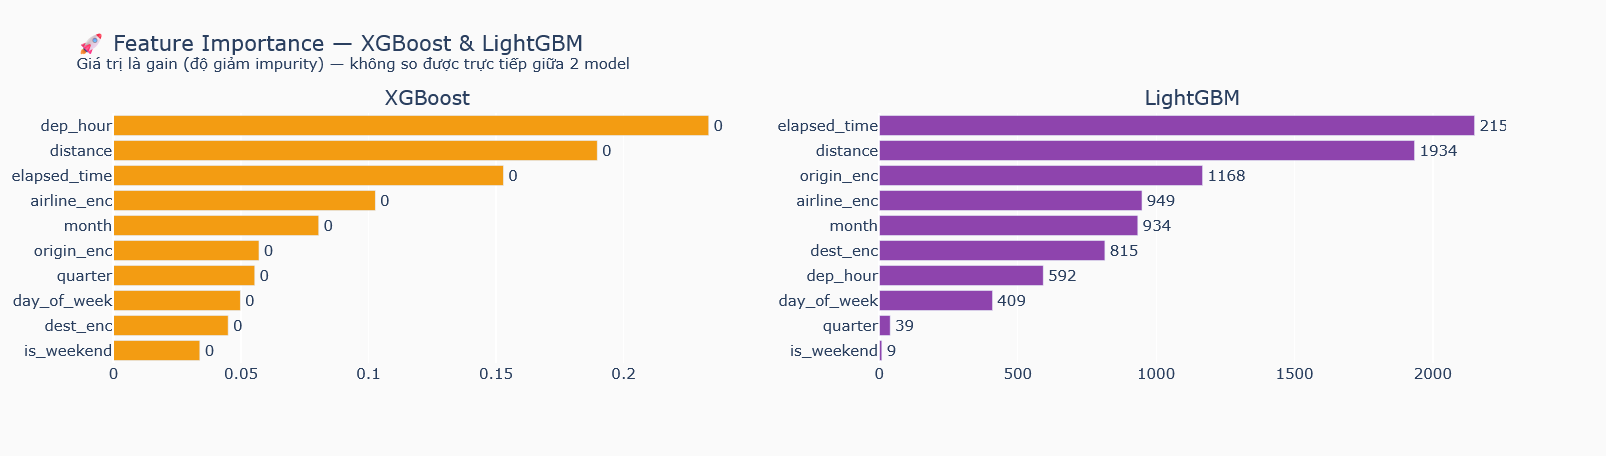
\includegraphics[width=0.75\textwidth]{img/feature_importance.png}
%     \caption{Feature Importance của mô hình LightGBM}
%     \label{fig:feature_importance}
% \end{figure}

\subsubsection{Phân tích tại sao Gradient Boosting thắng}

Các lý do Gradient Boosting (XGBoost/LightGBM) đạt hiệu suất tốt nhất:

\begin{enumerate}
    \item \textbf{Mô hình hóa phi tuyến phức tạp:} Quan hệ giữa delay và các đặc trưng (giờ bay,
          hãng bay, sân bay) không tuyến tính --- Logistic Regression không bắt được điều này.

    \item \textbf{Xử lý interaction features tự nhiên:} GBDT tự tạo các điều kiện kết hợp
          (ví dụ: hãng F9 \textit{và} tháng 12 \textit{và} sân bay ORD) mà không cần feature engineering tay.

    \item \textbf{Khả năng chống overfitting tốt hơn Random Forest:}
          Boosting sequential correction cho phép cây nhỏ (shallow) kết hợp với nhau hiệu quả,
          trong khi Random Forest cần cây sâu hơn để đạt độ chính xác tương đương.

    \item \textbf{Xử lý mất cân bằng lớp hiệu quả:}
          \texttt{scale\_pos\_weight} của XGBoost và \texttt{is\_unbalance} của LightGBM
          được thiết kế đặc biệt cho bài toán imbalanced classification.

    \item \textbf{LightGBM nhanh nhất trong nhóm:} Leaf-wise growth + GOSS sampling
          giúp LightGBM huấn luyện nhanh hơn XGBoost \textasciitilde{}2--5 lần với AUC tương đương.
\end{enumerate}

% ------------------------------------------------------------
\subsection{Thảo luận}

\subsubsection{Giải quyết được vấn đề gì?}

So sánh với mục tiêu ban đầu:
\begin{itemize}
    \item[$\checkmark$] \textbf{Data Warehouse:} Đã xây dựng thành công, lưu trữ toàn bộ 5,8M chuyến bay
          trong SQLite với Star Schema, hỗ trợ truy vấn OLAP linh hoạt.
    \item[$\checkmark$] \textbf{Dashboard OLAP:} Giao diện 2 cấp cung cấp insight về nguyên nhân,
          thời điểm và tác nhân delay, thay thế hoàn toàn phân tích thủ công.
    \item[$\checkmark$] \textbf{Dự báo delay:} Mô hình đạt AUC $\approx$ 0,73 --- tốt hơn baseline
          ngẫu nhiên (0,5) một cách đáng kể, có thể triển khai trong hệ thống cảnh báo sớm.
\end{itemize}

\subsubsection{Những trường hợp model còn sai và tại sao}

Mô hình có xu hướng dự đoán sai trong các trường hợp:
\begin{itemize}
    \item \textbf{Delay đột xuất do thời tiết cực đoan:} Bão tuyết bất ngờ, mưa đá không dự báo được
          từ dữ liệu lịch sử --- model không có feature thời tiết thực tế.
    \item \textbf{Chuyến bay đầu tiên trong ngày:} \texttt{DEPARTURE\_DELAY} = 0 nhưng thực tế delay
          do lý do vận hành nội bộ của hãng (thiếu phi hành đoàn, bảo trì kỹ thuật đột xuất).
    \item \textbf{Sân bay và hãng ít dữ liệu:} Một số sân bay nhỏ/hãng nhỏ có ít mẫu huấn luyện,
          dẫn đến encoding không đại diện.
    \item \textbf{Ngày lễ đặc biệt:} Thanksgiving, Giáng sinh có hành vi delay đặc biệt khác với
          các ngày thường trong cùng tháng --- model chưa bắt được hiệu ứng này.
\end{itemize}

% ============================================================
% CHƯƠNG 5: KẾT LUẬN VÀ HƯỚNG PHÁT TRIỂN
% ============================================================
\clearpage
\section{Kết luận và hướng phát triển}

% ============================================================
\subsection{Kết luận}

\subsubsection{Đánh giá mức hoàn thành so với mục tiêu}

Đề tài đặt ra ba mục tiêu ban đầu; bảng dưới đây đối chiếu
từng mục tiêu với kết quả đạt được:

\begin{enumerate}
    \item \textbf{Data Warehouse chuẩn hóa.}
    Kho dữ liệu SQLite theo Star Schema đã được xây dựng hoàn chỉnh:
    1 bảng sự kiện (\texttt{fact\_flights}, $\approx$5{,}3M bản ghi),
    4 bảng chiều và 6 chỉ mục OLAP.
    ETL pipeline streaming kết hợp tối ưu dtype (\texttt{float32}/\texttt{int8})
    giữ RAM ổn định $\approx$120\,MB/chunk, hoàn thành trong 3--8 phút ---
    chứng minh kiến trúc phân lô hoạt động hiệu quả trên máy cá nhân.

    \item \textbf{Dashboard OLAP đa chiều.}
    Dashboard Streamlit 6 trang (Tổng quan, Tuyến đường, Thời gian,
    Nguyên nhân, Dự báo, Explorer) kết hợp Plotly,
    hiện thực đầy đủ các phép OLAP (Slice, Dice, Roll-up, Drill-down)
    thông qua bộ lọc tương tác theo tháng/quý, hãng và địa lý.
    Mỗi trang tập trung một góc nhìn phân tích riêng,
    giúp người dùng khám phá dữ liệu một cách có hệ thống.

    \item \textbf{Mô hình dự báo delay.}
    Framework so sánh 5 thuật toán (Logistic Regression, Random Forest,
    Neural Network, XGBoost, LightGBM) trên cùng tập dữ liệu và 7 chỉ số.
    Mô hình tốt nhất (XGBoost) đạt AUC-ROC $\approx$ 0{,}75 ---
    vượt đáng kể so với baseline ngẫu nhiên (0{,}5) --- với bộ feature
    hoàn toàn ``dự báo''.
\end{enumerate}

% ------------------------------------------------------------
\subsubsection{Insight thực tế và khuyến nghị từ dữ liệu 2015}

Kết hợp phân tích OLAP trên dashboard và Feature Importance từ mô hình,
nhóm rút ra các quy luật quan trọng, kèm \textbf{khuyến nghị hành động}
cho các bên liên quan:

\begin{itemize}
    \item \textbf{Hiệu ứng dây chuyền là nguyên nhân delay lớn nhất.}
          Late Aircraft và NAS chiếm tỷ trọng trễ cao nhất ---
          hệ thống hàng không rất nhạy với gián đoạn ban đầu:
          một chuyến delay buổi sáng có thể lan sang 3--5 chuyến tiếp theo.
          \textit{Khuyến nghị cho hãng:} tăng buffer thời gian quay đầu tàu bay
          (\textit{turnaround time}) cho các chuyến nối tiếp,
          đặc biệt tại sân bay hub.

    \item \textbf{Mùa hè (tháng 6--7) và mùa đông (tháng 12--1) là hai đỉnh delay.}
          Trùng với mùa bão và mùa tuyết --- hai giai đoạn mà tỷ lệ trễ
          vượt trung bình năm đáng kể.
          \textit{Khuyến nghị cho quản lý sân bay:} chuẩn bị phương án
          dự phòng vận hành riêng cho hai mùa cao điểm,
          bao gồm bổ sung nhân lực mặt đất và tối ưu lịch bay.

    \item \textbf{Chuyến sáng sớm (trước 8h) ít delay nhất.}
          Chưa chịu ảnh hưởng tích lũy từ các trễ trong ngày.
          \textit{Khuyến nghị cho hành khách:} ưu tiên chuyến sáng sớm
          nếu cần đảm bảo đúng giờ cho kết nối quan trọng.

    \item \textbf{Hãng bay ảnh hưởng có hệ thống đến đúng giờ.}
          Chênh lệch OTP giữa hãng tốt nhất và kém nhất lên đến 15--20 điểm phần trăm,
          phản ánh khác biệt trong chiến lược quay đầu, bảo trì và xếp lịch.
          \textit{Khuyến nghị cho ngành:} benchmark OTP công khai
          tạo áp lực cải thiện từ phía hãng có tỷ lệ trễ cao.

    \item \textbf{Quãng đường và thời gian bay là feature quan trọng nhất trong mô hình.}
          Chuyến bay dài chịu nhiều rủi ro hơn (thời tiết, không phận, tiêu thụ nhiên liệu).
          Yếu tố địa lý (bang sân bay) cũng được mô hình khai thác mạnh,
          cho thấy hạ tầng và khí hậu vùng miền là nhân tố phân biệt rõ.
\end{itemize}

% ============================================================
\subsection{Hạn chế}

\begin{enumerate}
    \item \textbf{Dữ liệu chỉ bao phủ năm 2015.}
    Insight và mô hình phản ánh thực trạng một năm cụ thể.
    Sự thay đổi về cơ sở hạ tầng, quy định FAA,
    và hành vi di chuyển sau đại dịch COVID-19
    có thể làm mô hình không còn phù hợp với thực tế hiện tại.
    Tuy nhiên, \textit{phương pháp luận} (kiến trúc DW, pipeline so sánh mô hình)
    vẫn áp dụng được khi thay đổi nguồn dữ liệu.

    \item \textbf{SQLite không phù hợp cho production.}
    SQLite là single-writer, không hỗ trợ concurrent access
    và không có cơ chế phân tán.
    Một số OLAP query phức tạp mất vài giây ---
    chấp nhận được cho đồ án nhưng không đủ cho hệ thống thực
    phục vụ nhiều người dùng đồng thời.

    \item \textbf{AUC-ROC $\approx$ 0{,}75 --- còn khoảng cách so với mô hình lý tưởng.}
    Mô hình chủ động \textbf{không dùng \texttt{departure\_delay}}
    để đảm bảo tính dự báo (trước khi cất cánh).
    Đổi lại, AUC bị giới hạn vì thiếu dữ liệu thời tiết thực tế,
    thông tin bảo trì tàu bay, và lịch sử delay từng tail number ---
    các yếu tố có thể cải thiện AUC thêm 0{,}03--0{,}10.

    \item \textbf{Chưa có Clustering / Association Rules.}
    Đề tài tập trung vào classification (dự báo delay)
    và OLAP (phân tích đa chiều).
    Các kỹ thuật khai phá khác như phân cụm sân bay theo hành vi delay
    hoặc luật kết hợp (``hãng A + sân bay ORD + tháng 12 $\Rightarrow$ delay'')
    chưa được thực hiện --- có thể là hướng bổ sung.
\end{enumerate}

% ============================================================
\subsection{Hướng phát triển}

\begin{enumerate}
    \item \textbf{Mở rộng dữ liệu nhiều năm.}
    Tích hợp dữ liệu 2010--2023 từ Bureau of Transportation Statistics (BTS)
    để phát hiện xu hướng dài hạn, đánh giá ảnh hưởng COVID-19 (2020--2021),
    và huấn luyện mô hình tổng quát hơn trên phân phối đa dạng.

    \item \textbf{Tích hợp dữ liệu thời tiết.}
    Kết hợp dữ liệu NOAA (nhiệt độ, lượng mưa, tốc độ gió)
    theo sân bay và ngày --- đây là yếu tố delay lớn nhất
    mà mô hình hiện tại chưa có.

    \item \textbf{Nâng cấp hạ tầng lưu trữ.}
    \begin{itemize}
        \item Thay SQLite bằng \textbf{PostgreSQL} hoặc \textbf{ClickHouse}
              để hỗ trợ concurrent access và OLAP query nhanh hơn.
        \item Containerize hệ thống bằng \textbf{Docker},
              deploy dashboard lên cloud (AWS EC2 / Google Cloud Run).
        \item Xây dựng \textbf{REST API} (FastAPI) cho dự báo delay
              theo yêu cầu thời gian thực.
    \end{itemize}

    \item \textbf{Giải thích mô hình với SHAP.}
    Áp dụng SHAP (SHapley Additive exPlanations) \cite{lundberg2017shap}
    để giải thích \textit{từng dự báo cụ thể}:
    tại sao chuyến bay này bị dự báo delay? Feature nào đóng góp nhiều nhất?
    Dashboard có thể hiển thị không chỉ ``có delay'' mà còn ``tại sao delay''.

    \item \textbf{Pipeline streaming thời gian thực.}
    Sử dụng Apache Kafka nhận dữ liệu chuyến bay real-time từ API hàng không,
    kết hợp Spark Streaming để dự báo delay ngay khi chuyến bay được đặt lịch ---
    chuyển hệ thống từ phân tích lịch sử sang hỗ trợ quyết định tức thời.
\end{enumerate}


% References
\cleardoublepage
\phantomsection
\addcontentsline{toc}{section}{Tài liệu tham khảo}
\bibliographystyle{plain}
\bibliography{ref/ref}
\end{document}